% !Mode:: "TeX:UTF-8"
%!TEX program  = xelatex

%\documentclass[bwprint]{cumcmthesis}
\documentclass[withoutpreface,bwprint]{cumcmthesis} %去掉封面与编号页

\title{葡萄酒的评价}
\tihao{B}
\baominghao{201723003xxx}
\schoolname{电子科技大学}
\membera{卫佳杰}
\memberb{谢沁余}
\memberc{任彦璟}
\supervisor{覃思义}
\yearinput{2017}
\monthinput{08}
\dayinput{23}

\begin{document}
 \maketitle
\begin{abstract}
\par 本文评价了两组评酒师的打分,并基于理论指标对葡萄酒质量进行了分析。
\par 本文首先验证了两组评价者对红白葡萄酒的评分均服从正态分布,在置信度为0.05的条件下,采用F检验针对每个样品组评酒师的总分进行方差齐性的假设检验,通过检验得出两组评酒员评价结果具有显著差异。基于评酒师均专业的假设,本文给出基于组内与组间差距的评价指标,并解得第一组评价结果更可信。

\par 本文对酿酒葡萄的理化指标进行K-means聚类,然后用类内葡萄酒的打分均值给等级排序,并依据类间样本尽可能分散,类内样本尽可能聚拢的准则通过Fisher函数选择分类个数。以白葡萄酒为例,得出等级一:样本27;等级二:样本5、7、15、20、24;等级三:样本3、6、10、12、13、18、28;等级四:样本1、2、4、9、14、21、23、25、26;等级五:样本 8、11、16、17、19、22。  

\par  本文将对酿酒葡萄的一级理化指标进行主成分分析后得到的主成分作为自变量,葡萄酒的一级理化指标作为因变量,进行多元回归分析,再通过迭代将主成分代回为酿酒葡萄的一级理化指标,最终得出葡萄酒与酿酒葡萄的理化指标之间的关系。

\par 最后本文将对酿酒葡萄和葡萄酒的一级理化指标进行主成分分析后得到的主成分作为自变量,评酒员打分作为因变量,进行多元线形回归,以白葡萄为例得出葡萄酒质量与理化指标主成分之间的关系,并通过回归检验的方法,得出相关系数$r^2=0.6455$、$F=4.0252$、与$F$对应的概率$p=0.0071$,$\sigma^2=6.4161$,其中与F对应的概率$p=0.007<0.05$,回归模型成立,并通过交叉检验模型检验得平均相对误差4.7\%,因此用葡萄和葡萄酒的理化指标可以评价葡萄酒的质量。
 
\keywords{F检验\quad  K-means聚类 \quad Fisher准则函数\quad  主成分分析\quad  多元线形回归 \quad 交叉检验}
\end{abstract}
\tableofcontents
\newpage

\section{问题重述}

\subsection{引言}

\par 本文将定性定量地讨论葡萄酒的质量问题。确定葡萄酒质量时一般是通过聘请一批有资质的评酒员进行品评。每个评酒员在对葡萄酒进行品尝后对其分类指标打分,然后求和得到其总分,从而确定葡萄酒的质量。酿酒葡萄的好坏与所酿葡萄酒的质量有直接的关系,葡萄酒和酿酒葡萄检测的理化指标会在一定程度上反映葡萄酒和葡萄的质量。附件1给出了某一年份一些葡萄酒的评价结果,附件2和附件3分别给出了该年份这些葡萄酒的和酿酒葡萄的成分数据。
\subsection{问题的提出}

本文需要建立数学模型讨论以下4个问题:

\begin{enumerate}
  \item 分析附件1中两组评酒员的评价结果有无显著性差异,并判断哪一组结果更可信。
  \item 根据酿酒葡萄的理化指标和葡萄酒的质量对这些酿酒葡萄进行分级。
  \item 分析酿酒葡萄与葡萄酒的理化指标之间的联系。
  \item 分析酿酒葡萄和葡萄酒的理化指标对葡萄酒质量的影响,并论证用葡萄和葡萄酒的理化指标来评价葡萄酒的质量的可行性。
\end{enumerate}


\section{问题分析}

\par 本题要求我们对题中给出的两组评酒员对相同的一批酒(27种红葡萄酒,28种白葡萄酒)的打分情况进行分析。

\subsection{问题一:两组评酒员打分问题的分析}

\par 本文首先分析两组评价结果是否具有显著的差异性,然后分析哪一组数据的可信度更高。通过数据分析,例如表(\ref{红葡萄酒第二组样品1正态检验})所示,可得出评酒员对每一种酒的评价总分基本服从正态分布。


\begin{table}
\centering
\caption{红葡萄酒第二组样品1正态检验}
\label{红葡萄酒第二组样品1正态检验}
\begin{tabular}{l|c}
\toprule
  个案数 & 10 \\
 正态参数 $\quad$ 平均值 & 68.1000  \\
 正态参数 $\quad$ 标准差 & 9.04863\\
 最极端差值	$\quad$绝对	&.252\\
最极端差值	$\quad$正	&.152\\
最极端差值	$\quad$负	&-.252\\
检验统计		$\quad$& .252\\
渐近显著性(双尾)		$\quad$& .072\\
\bottomrule
\end{tabular}

\end{table}


因此本文选用抽样分布定理中的$T$假设检验对两组样本的均值进行检验,并用$F$检验对两组样本的方差进行检验,得出两组样品的得分是否具有显著性差异。
\par 在评价两组评酒员评价红、⽩两种葡萄酒时的评价可信度时,基于评酒员均为专业⼈⼠的假设下,可认为他们对某种酒的评价的方差和极差越小、打分越趋于一致,则说明对于某种酒的评价越可信。

\subsection{问题二:对酿酒葡萄的分级问题}

\par 首先题目中提到酿酒葡萄的好坏与所酿葡萄酒的质量有直接的关系,而酿酒葡萄的理化指标决定了酿酒葡萄质量的好坏,因此本文采用无监督K-means聚类方法,将红葡萄酒与白葡萄酒分别聚类为3、4、5类,之后通过Fisher准则函数对三种分类情况进行计算,选取其中分类性好的分类数作为本文对酿酒葡萄的分类个数。最终分别得出红葡萄酒和白葡萄酒的酿酒葡萄的等级。

\subsection{问题三:酿酒葡萄与葡萄酒的理化指标的联系}


\par 本文定义葡萄的质量对葡萄酒的质量影响是直接的,而酿酒葡萄的质量受酿酒葡萄理化指标的决定,葡萄酒的质量受到葡萄酒理化指标的决定(关系如图(\ref{酿酒葡萄与葡萄酒的理化指标的联系})所示),因此我们通过多元回归分析得出酿酒葡萄的理化指标与葡萄酒每个主要的理化指标之间的关系。

\subsection{问题四:酿酒葡萄和葡萄酒的理化指标对葡萄酒质量的影响分析}

\par 本文将酿酒葡萄的理化指标与葡萄酒的理化指标作为自变量,葡萄酒的质量我们用第一问中可行度更高的一组的评分来替代作为因变量,通过多元线性回归,得出理化指标与葡萄酒质量之间的关系。为了验证葡萄和葡萄酒的理化指标来评价葡萄酒的质量的合理性,本文划分样本集,最后通过回归检验来评价这种方法的可行性。 

\section{模型的假设}

\begin{enumerate}
	\item 两组评酒员进行打分的(27种红葡萄酒,28种白葡萄酒)是相同的一批酒。
	\item 其中一组评酒员的评价总分能较为客观和稳定地反映葡萄酒的质量。
	\item 芳香物质归并入理化指标中的子项。
	\item 葡萄酒和酿酒葡萄检测的理化指标会在一定程度上反映葡萄酒和葡萄的质量。
	\item 酿酒葡萄的好坏与所酿葡萄酒的质量有直接的关系。
\end{enumerate}

\section{符号说明}
\begin{table}[!h]
\centering
\begin{tabular}{cc}

\toprule
 \makebox[0.4\textwidth][c]{符号}	&  \makebox[0.5\textwidth][c]{意义} \\ \midrule
 $Y$	& 葡萄酒质量 \\ 
 $X_i$	    & 理化指标和芳香物质综合得到的主成分  \\ 
\bottomrule 
\end{tabular}
\end{table}

\section{建模前准备}
\subsection{数据预处理}
\par 处理数据前,首先需要检查数据的完备性和合理性。
\par 例如,第一组红葡萄酒样品20中缺失品酒员4号对于外观分析中色调的评分,利用该组其他品酒师评分的均值6分进行填充。
\begin{figure}[!h]
\centering
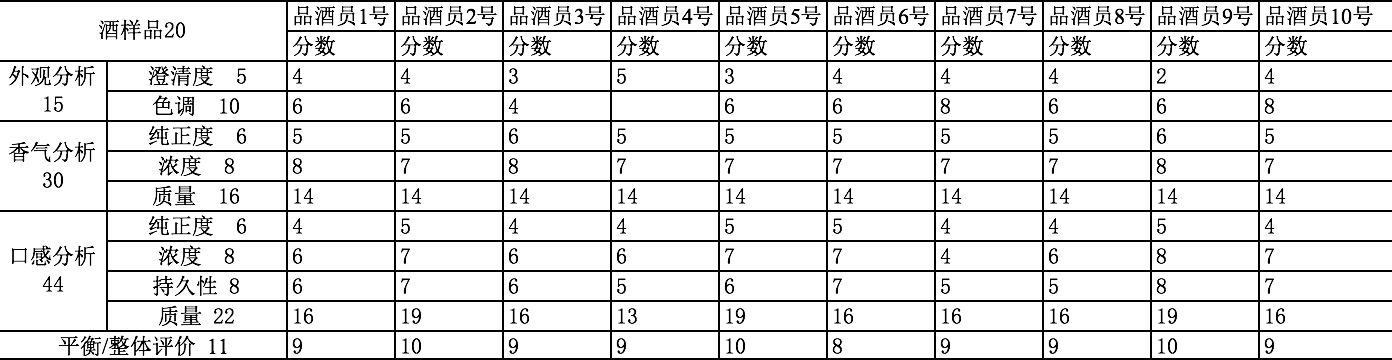
\includegraphics[width=\textwidth]{err1.png}
\caption{数据缺失}
\label{数据异常}
\end{figure}

第一组白葡萄酒样品3中品酒员7号对于口感分析中持久性的评分是77,为异常值,利用该组其他品酒师评分的均值6分进行替换。
\begin{figure}[!h]
\centering
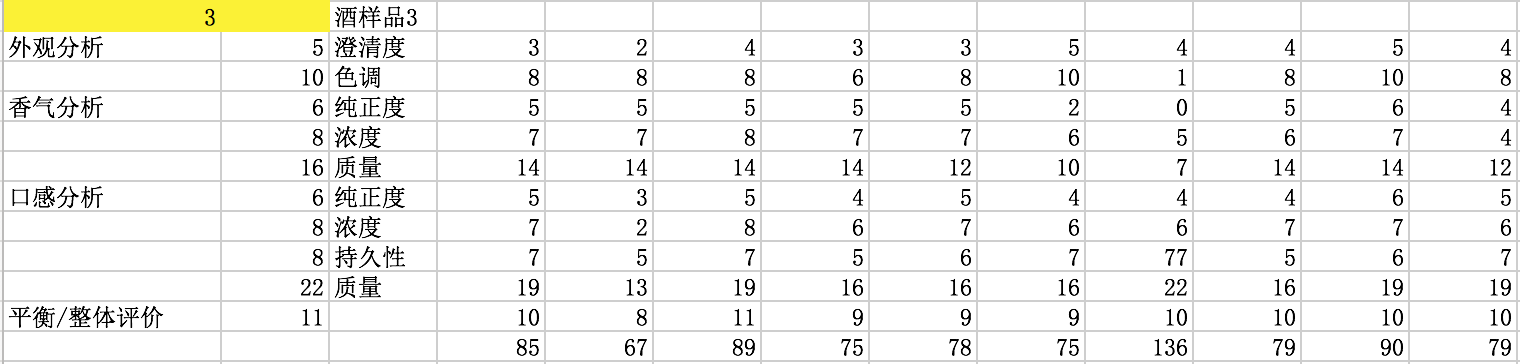
\includegraphics[width=\textwidth]{err2.png}
\caption{数据异常}
\label{数据异常}
\end{figure}

\subsection{数据归一化}
本文涉及大量数据,尤其附件二附件三包含多种理化指标的含量,单位不一,数据大小差异很大。因而需要归一化,以便进行后续处理。本文采用0均值标准化归一方法,将大多数指标控制在-4到4之间。
\begin{equation}
	x' = \frac{x - \bar{x}}{\sigma}
\end{equation}

其中$\sigma$表示样本标准差,$\bar{x}$表示样本均值,$x'$的取值范围是$(-\infty, \infty)$,但从经验上看,大多数取值范围在$[-4,4]$之间。

\section{问题一:两组评酒员打分问题}

\subsection{模型建立}
第一问要分析附件1中两组评酒员的评价结果有无显著性差异,并判断哪一组结果更可信。本题需要对题中给出了两组评酒员对相同的一批酒(27种红葡萄酒,28种白葡萄酒)的打分情况进行分析。首先,对于一个样品而言,本文将单个样品被单个评酒员评价的总分(外观分析+香气分析+口感分析+平衡/整体评价)作为一个品酒员对一个酒样品的评价结果。下述分数均代指总分。

对于显著性差异,本文通过F检验(方差齐性检验)进行判断。分别选取一、二两组同种同编号葡萄酒样品进行检验。基于问题分析中对于每一组评酒员对同意葡萄酒样品的评价总分呈现正态分布的检验结果(如表(\ref{红葡萄酒第二组样品1正态检验})),本文进行F检验如。

本文通过两个正态总体方差比$\sigma_1^2/\sigma_2^2$来检验方差齐性,采用双侧假设检验,原假设H0备择假设H1分别为:$H_0:\sigma_1^2= \sigma_2^2$,$H_1:\sigma_1^2 \neq \sigma_2^2$。
\begin{equation}
	\label{1-1-1}
	F = \frac{S_1^2/\sigma_1^2}{S_2^2/\sigma_2^2} = \frac{S_1^2}{S_2^2} \sim F(n_1 - 1, n_2 - 1)
\end{equation}

同时,定义如下公式(\ref{1-1-n})所示计算方法,认为参数$K$在满足公式时两组评酒员对葡萄酒的评价结果具有显著性差异,其中$\varepsilon$为显著性水平,一般取值$0.05$,$n$是全部样本的个数,$n_0$是两组评酒员对同一样品的评分在F检验中被拒绝的个数。

\begin{equation}
\label{1-1-n}
	K = \frac{n_0}{n} > \varepsilon
\end{equation}

针对两组评酒员评分可信度的分析,本文通过对任一个样品10个评酒员总分的方差,每组同类葡萄酒全部样本的平均方差$A$来刻画组内差距;求每组10个评酒员对同一样品评分的平均值,再将同组评酒员、同类葡萄酒的全部样品的前述平均值求方差$B$来刻画组间差距。最终通过指标$A/B$评价两组评酒员的评价可信度。

\subsection{模型求解}
\subsubsection{评价结果差异性}

由检验统计量公式(\ref{1-1-1})可得,对于评价哪组数据的可信度高这一问题,本文将其转化为评价的稳定性问题。对于同一个样品,理论上存在葡萄酒质量的真值,一组评酒师的评价可看作随机在真值附近波动的估计值。一组评酒师总分越一致,稳定性越高,方差越小。因而评酒师对某种酒的评价的方差越小,则说明该组品酒员的评价越可信。

对样品的显著性差异,利用F检验方差齐性,结果如下表(\ref{红葡萄酒F检验结果},\ref{白葡萄酒F检验结果})所示:

\begin{table}[!htbp]
\centering
\caption{红葡萄酒F检验结果}
\label{红葡萄酒F检验结果}
\begin{tabular}{lcccccccccccccc}
\toprule
样品	& 1 & 2 & 3 & 4 & 5 & 6 & 7 & 8 & 9 & 10 & 11 & 12 & 13 & 14\\
\midrule
F & 1.13 &2.45 &1.49 &2.62 &4.54 &2.83 &1.65 &1.48 &1.28 &1.19 &1.86 &3.17 &2.94 &1.56\\
差异 & 无 &无 &无 &无 &有 &无 &无 &无 &无 &无 &无 &无 &无 &无\\
\midrule
样品	  & 15 & 16 & 17 & 18 & 19 & 20 & 21 & 22 & 23 & 24 & 25 & 26 & 27 & \\
\midrule
F   &2.07 &1.11 &9.6 &1.06 &1.16 &1.50 &3.27 &2.09& 1.31 &6.98 &1.48 &1.33 &2.43 &\\
差异   &无 &有 &无 &无 &无 &无 & 无 &无 &有 &无 &无 &无 &无&\\
\bottomrule 
\end{tabular}
\end{table}

\begin{table}[!htbp]
\centering
\caption{白葡萄酒F检验结果}
\label{白葡萄酒F检验结果}
\begin{tabular}{lcccccccccccccc}
\toprule
样品	& 1 & 2 & 3 & 4 & 5 & 6 & 7 & 8 & 9 & 10 & 11 & 12 & 13 & 14\\
\midrule
F & 3.56 & 4.10 &2.56 &1.06 &4.81 &7.16 &1.08 & 5.90 &1.15 &3.02 &2.02 &1.21 &3.65 &7.91\\
差异 & 无 &有 &无 &无 &有 &有 &无 & 有 &无 &无 &无 &无 &无 &有\\
\midrule
样品	  & 15 & 16 & 17 & 18 & 19 & 20 & 21 & 22 & 23 & 24 & 25 & 26 & 27 & 28\\
\midrule
F   & 2.44 &2.16 &3.75 &5.18 &1.78 &1.29 &2.68 & 2.59 &3.76 &2.88 &3.14 &1.41 &4.06 &3.17\\
差异   & 无 &无 &无 &有 &无 &无 &无 & 无 &无 &无 &无 &无 &有 &无\\
\bottomrule 
\end{tabular}
\end{table}

对于红葡萄酒,其参数$=0.11>0.05$;对于白葡萄酒,其参数$K=0.26>0.05$。因此,可认为两组评酒员评价结果存在明显之差异。
\subsubsection{评价结果可信度}

对于同一个样品,本文分别求出两组评酒员总分的方差。对27种红葡萄酒,28种白葡萄酒就会产生(27+28)个方差比较,如下图(\ref{白葡萄酒评分方差},\ref{红葡萄酒评分方差})所示(其中点划线代表第一组,实线代表第二组):
\begin{figure}[!h]
\centering
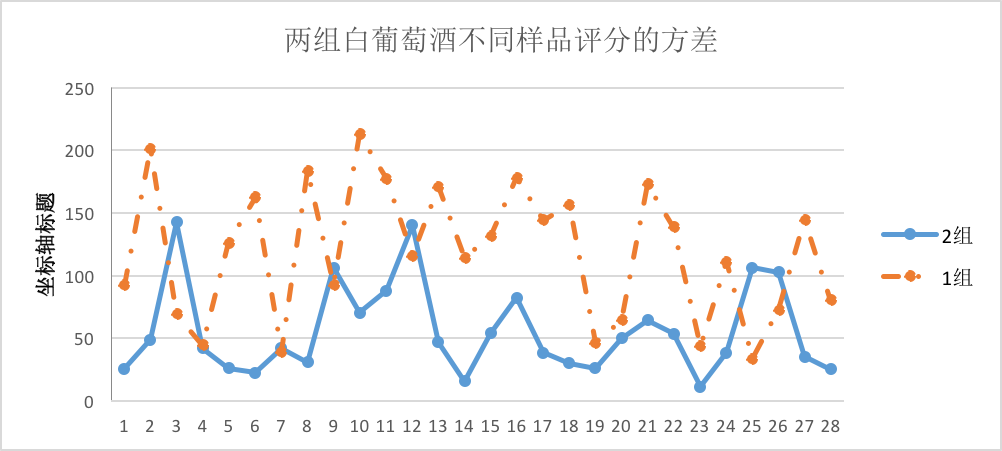
\includegraphics[width=\textwidth]{1-1.png}
\caption{白葡萄酒评分方差}
\label{白葡萄酒评分方差}
\end{figure}
\begin{figure}[!h]
\centering
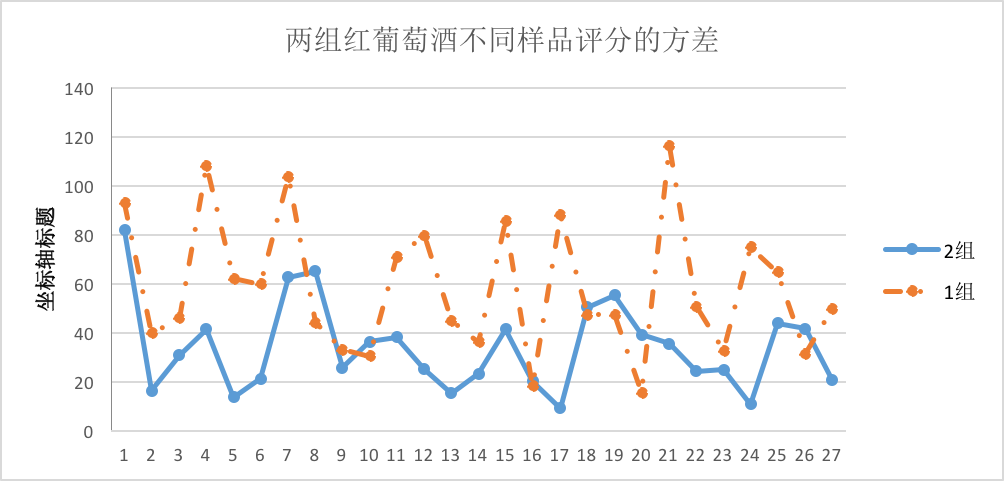
\includegraphics[width=\textwidth]{1-2.png}
\caption{红葡萄酒评分方差}
\label{红葡萄酒评分方差}
\end{figure}

计算结果如下表(\ref{可信度检验结果})所示:

\begin{table}[!htbp]
\centering
\caption{可信度检验结果}
\label{可信度检验结果}
\begin{tabular}{ccccc}
\toprule
组别 & 组内差距 & 组间差距 & 评价指标A/B\\
\midrule
第一组红葡萄酒 & 58.23 & 52.18  & 1.12\\

第一组白葡萄酒 & 118.62 & 22.22  & 5.34\\
第二组红葡萄酒 & 33.79 & 15.82 & 2.14\\
第二组白葡萄酒 & 56.2 & 10.05 &5.59\\
\bottomrule 
\end{tabular}
\end{table}


由可信度检验结果可得出,对于白葡萄酒,无论白葡萄酒或红葡萄酒,第一组评价指标均小于第二组,因此可认为第一组评酒员评价结果更可信。
\newpage
\section{问题二:酿酒葡萄分级问题}
\subsection{模型建立}

\par 由于酿酒葡萄啊理化指标的变量数太多,我们为简化计算,通过对酿酒葡萄理化指标进行主成分分析,并采用每一个主成分的贡献度作为主成分的权重,对每个样品进行打分,并通过归一化的逆过程,将打分结果的变化范围确定在0-100分。最后用主成分分析得到的分值与每种样品葡萄酒质量评分进行无监督K-means聚类的方法,将红葡萄酒与白葡萄酒分别聚成若干类,再通过聚类后葡萄酒评分的均值分出酿酒葡萄的等级。由于在使用K-means聚类算法事先不确定k的值,因此我们通过分别选取k=3,k=4,k=5,即将某种酿酒葡萄的理化指标分成三类、四类、五类、这些较为合理的分类数,之后通过Fisher准则函数对三种分类情况进行计算,选取其中分类性好的分类数作为本文对酿酒葡萄的分类个数。最终分别得出红葡萄酒和白葡萄酒的酿酒葡萄的等级。

\subsubsection{主成分分析法\upcite{主成分分析}}
\par 基本原理:假定有n个样本,每个样本有p个变量,构成一个n*p阶的数据矩阵,如公示(\ref{Xarry})所示。

\begin{equation}
\label{Xarry}
X = \begin{bmatrix}
x_{11} & x_{12} & \cdots & x_{1p}\\
x_{21} & x_{22} & \cdots & x_{2p}\\
\vdots & \vdots & \ddots & \vdots \\
x_{n1} & x_{n2} & \cdots & x_{np}\\
\end{bmatrix}
\end{equation}


\par 当$p$较大时,在$p$维空间中考察问题比较麻烦。为了克服这一问题,就需要进行降维处理,即用较少的几个综合指标代替原有较多的变量的指标,而且使这些较少的综合指标既能尽量多的反应原来较多变量指标所反应的信息,同时他们之间又是彼此相互独立的。

\par 定义:记$x_1,x_2,x_3,\cdots,x_p$为原变量指标,$z_1,z_2,\cdots ,z_m \quad (m \leqslant p)$为新变量指标。

\begin{equation}
\label{zz}
\left\{
\begin{aligned}
z_1 = l_{11}x_1 + l_{12}x_2 + \cdots + l_{1p}x_p\\
z_2 = l_{21}x_1 + l_{22}x_2 + \cdots + l_{2p}x_p\\
\cdots \cdots \cdots \\
z_m = l_{m1}x_1 + l_{m2}x_2 + \cdots + l_{mp}x_p
\end{aligned}
\right.
\end{equation}

\textbf{系数的确定}
\par (1)每个主成分的系数的平方和为1。如公式(\ref{系数1})所示:

\begin{equation}
\label{系数1}
	l_{i1}^{2} + l_{i2}^{2} + \cdots + l_{ip}^{2} = 1
\end{equation}

\par (2)主成分之间相互独立,即无重叠的信息,即

\begin{equation}
	cov(z_i,z_j) = 0, \quad i \neq j ,\quad i,j = 1,2,\cdots,p
\end{equation}
\par (3)主成分的方差依次递减,重要性依次递减
\begin{equation}
	Var(z_1) \geqslant Var(z_2) \geqslant \cdots \geqslant Var(z_m)   	
\end{equation}

\par 通过以上分析我们可以看出,主成分分析的实质就是就是确定原来的变量在各主成分上的荷载。从数学关系上可以证明,这些荷载分别是相关性矩阵$m$个较大特征值所对应的特征向量。

\subsubsection{K-means聚类模型\upcite{k-means}}
\textbf{算法原理}
\par 给定样本集$D=\{x_1,x_2,\cdots,x_m\}$,$K-means$算法针对聚类所得到的簇划分$C=\{C_1,C_2,\cdots,C_k\}$最小化平方误差,即该目标函数为:
\begin{equation}
	E = \sum\limits_{i=1}^{k} \sum\limits_{x \in C_i} \mid x-\mu_i \mid ^2
\end{equation}

\par 其中x是簇$C_i$的新均值向量,$\mu_i$是簇的前一个均值向量。

\textbf{算法步骤}
\begin{enumerate}
	\item 在样本集中随机选取k个样本作为初始的均值向量$\{\mu_1,\mu_2,\cdots,\mu_k\}$。
	\item 计算样本$x_j$与各均值向量$(1 \leqslant i \leqslant k)$的距离。
	\item 根据与$x_j$距离最近的均值向量确定$x_j$的簇标记。
	\item 将样本$x_j$与$x_j$距离最近的均值向量划分为新的簇。
	\item 根据聚好的类别重新计算每一类的均值向量,与前述均值向量对比,如果不一样,则继续重复2,3,4的过程。如果相同则聚类结束。
\end{enumerate}
\textbf{算法思想}
\par $K-means$采用贪心策略,通过迭代求解。先随机选取$K$个样本作为 将要产生$k$类的中心,然后对其余的样本点进行聚类,得到$K$个类,从新计算每个类的中心,观察是否与之前选取的中心一致,若一致则这个聚类模型较为稳定,当且仅当有一个中心不一致,继续选取新的中心作为将产生新的$k$类的新中心,不断迭代,直到所有中心一致。
\subsubsection{$Fisher$准则函数\upcite{Fisher}}
$$
	J = \frac{\frac{1}{k}\sum\limits_{i<j}^{k}(\mu_i-\mu_j)^2	}{\frac{1}{k}\sum\limits_{i=1}^{k}\sum\limits_{m=1}^{n} (\sigma_{im}\sigma_{i0})^2}
$$

\begin{equation}
\label{Fisher2}
	J = \frac{\sum\limits_{i<j}^{k}(\mu_i-\mu_j)^2}{\sum\limits_{i=1}^{k}\sum\limits_{m=1}^{n}(\sigma_{im}\sigma_{i0})^2}
\end{equation}

\par 如公式(\ref{Fisher2})所示,$Fisher$准则函数的分子表示类与类之间的分散程度使用类与类距离的平方和的均值来刻画。分母表示类中样本的聚合程度使用样本与类中心的距离的平方和的均值来刻画。

\par 本文判别分出类的个数的判别基本思想是将数据的统计性质—均值与离散度的函数,作为判别分类优劣的标准。即:
\begin{enumerate}
	\item 分出的若干类之间的距离尽可能远。
	\item 每一类之中的样本尽可能紧凑。
\end{enumerate}

\par 因此$Fisher$函数值越大表明分类的效果越好,我们希望$Fisher$函数值越大越好。因此将$K-means$的三类、四类、五类聚类结果结果分别带入验证,选出$Fisher$准则函数最大的值对应类的个数作为分类的类别数。

\subsection{模型求解}

\par 为了建立酿酒葡萄质量等级较为客观的模型,我们将酿酒葡萄的理化指标进行主成分分析并打分,将通过主成分分析的打分与评酒员对酒的评分同时作为葡萄酒质量的评价指标并聚类,并将每组这两个评分的均值的高低作为等级的高低。

\par 以红葡萄酒为例展示结果。
\subsubsection{进行主成分分析并确定主成分}
\begin{table}[!htbp]
\centering
\caption{主成分分析结果}
\label{主成分分析结果}
\begin{tabular}{ccccc}
\toprule
 & 主成分累计贡献度(\%) & 主成分贡献度(\%)\\
\midrule
F1&23.221&23.22066957\\
F2&39.687&16.4667406354233\\ 
F3&52.144&12.4570051467150\\ 
F4&61.611&9.4667525243561\\ 
F5&68.274&6.6627744799786\\ 
F6&74.082&5.8078512959928\\ 
F7&78.810&4.7281727290170\\ 
F8&83.044&4.2335398181635\\ 
\bottomrule 
\end{tabular}
\end{table}

\subsubsection{主成分进行打分并且得到综合得分}
\begin{equation}
\label{2-1-s}
	S_{coer} = F_1 * \alpha_1 + \cdots + F_k*\alpha_k
\end{equation}
公式(\ref{2-1-s})中$S_{coer}$为综合分,$F_1,\cdots,F_k$为k个主成分,$\alpha_1,\cdots,\alpha_k$为k个主成分对应的权重值。如下表(\ref{通过主成分对红葡萄打分结果})所示,为部分结果。

\begin{table}[!htbp]
\centering
\caption{通过主成分对红葡萄打分结果}
\label{通过主成分对红葡萄打分结果}
\begin{tabular}{cccccccccc}
\toprule
 &F1&F2&F3&F4&F5&F6&F7&F8&综合打分\\
\midrule
样本1&1.7934&0.3900&0.0279&-1.901&0.3221&1.8674&-1.807&0.5428&37.156\\
样本2&1.6832&-0.423&0.1332&0.6341&0.6162&0.0067&-1.598&0.3818&37.973\\
样本3&1.6605&1.4381&-0.241&1.8009&-0.955&-1.902&0.8051&1.2175&67.821\\
样本4&-0.887&0.2436&0.0383&-0.214&-0.716&-0.124&-0.354&-0.564&-27.71\\
样本5&-0.109&-0.626&-0.659&0.4090&1.6816&0.1766&0.7446&-0.281&-2.633\\
样本6&-0.403&1.2245&-1.318&0.3231&-0.536&0.4969&-0.149&0.5451&-1.666\\
\bottomrule 
\end{tabular}
\end{table}



\subsubsection{将综合得分进行标准化成百分制的形式}
\begin{equation}
\label{2-1-s'}
	S'=\frac{S_{core}-min}{max-min}\times 100
\end{equation}
通过公式(\ref{2-1-s'})进行标准化,部分结果如下表(\ref{通过最大值最小值标准化成百分制的结果})所示。
\begin{table}[!htbp]
\centering
\caption{通过最大值最小值标准化成百分制的结果}
\label{通过最大值最小值标准化成百分制的结果}
\begin{tabular}{cccccccccc}
\toprule
 &综合评分&主成分标准化得分\\
\midrule
样本1&37.15622&76.03093855\\
样本2&37.97394&76.61703959\\
样本3&67.82191&98.01045504\\
样本4&-27.714&29.53548642\\
样本5&-2.63347&47.51183187\\
样本6&-1.66693&48.20459491\\
\bottomrule 
\end{tabular}
\end{table}

\subsubsection{通过K-means聚类得出聚出的类别}
对主成分标准化得分和评酒员打分均值这两个维度的指标进行K-means聚类,得到结果如下表(\ref{K-means聚类非完整表})所示(非完整)。
\begin{table}[!htbp]
\centering
\caption{K-means聚类非完整表}
\label{K-means聚类非完整表}
\begin{tabular}{cccccccccc}
\toprule
 &主成分标准化得分&评酒员打分均值\\
\midrule
样本1&76.03093855&62.7\\
样本2&76.61703959&80.3\\
样本3&98.01045504&80.4\\
样本4&29.53548642&68.6\\
样本5&47.51183187&73.3\\
样本6&48.20459491&72.2\\
\bottomrule 
\end{tabular}
\end{table}

\par 经过Fisher函数检验,结果如下表(\ref{Fisher函数检验})所示。
\begin{table}[!htbp]
\centering
\caption{Fisher函数检验结果}
\label{Fisher函数检验}
\begin{tabular}{cccccccccc}
\toprule
 &分3类&分4类&分5类\\
\midrule
Fisher函数&5.6776&2.7989&7.0919\\
\bottomrule 
\end{tabular}
\end{table}

\subsubsection{通过两个打分的均值确定酿酒葡萄质量等级}
因此我们选取分5类的结果并通过两个打分结果求平均可以得到等级以及对应的样品
。结果如下表(\ref{红葡萄酒质量分级结果},\ref{白葡萄酒质量分级结果})所示。
\begin{table}[!htbp]
\centering
\caption{红葡萄酒质量分级结果}
\label{红葡萄酒质量分级结果}
\begin{tabular}{ll}
\toprule
 酿酒红葡萄等级&酿酒红葡萄样品\\
\midrule
第一等级(最高等级)&3、9、11\\
第二等级&1、2、21、22、23\\
第三等级&4、5、6、7、8、14、15、16、17、18、19、20、24\\
第四等级&12\\
第五等级&10、25、26、27\\
\bottomrule 
\end{tabular}
\end{table}

\begin{table}[!htbp]
\centering
\caption{白葡萄酒质量分级结果}
\label{白葡萄酒质量分级结果}
\begin{tabular}{ll}
\toprule
酿酒白葡萄等级&酿酒白葡萄样品\\
\midrule
第一等级(最高等级)&27\\
第二等级&5、7、15、20、24\\
第三等级&3、6、10、12、13、18、28\\
第四等级&1、2、4、9、14、21、23、25、26\\
第五等级&8、11、16、17、19、22\\
\bottomrule 
\end{tabular}
\end{table}



\newpage
\section{问题三:酿酒葡萄与葡萄酒的理化指标的联系}
\subsection{模型建立}
\par 针对第三问,本文采用多元线性回归来建立酿酒葡萄与葡萄酒的理化指标的联系。因为酿酒葡萄和葡萄酒的理化指标比较多,本文只考虑酿酒葡萄与葡萄酒的一级理化指标。由于酿酒葡萄的一级理化指标也有30种,考虑到自变量过多不利于回归分析而且这30个理化指标相互之间也有关联,需要进行自变量的筛选。对每一类葡萄酒的一级理化指标,都先计算酿酒葡萄30个一级理化指标和它的相关系数,在置信度0.05下将相关系数小的自变量忽略掉。最后将酿酒葡萄的每一个一级理化指标作为因变量,筛选后的酿酒葡萄的一级理化指标作为自变量进行多元线性回归。最终得到每一个回归方程的回归系数,相关系数$r^2$和与F对应的概率p。相关系数$r^2$越接近1,说明回归方程越显著。概率$p<0.05$时,回归模型成立。
\subsubsection{相关系数}
\par 相关系数是用以反映变量之间相关关系密切程度的统计指标。相关系数是按积差方法计算,同样以两变量与各自平均值的离差为基础,通过两个离差相乘来反映两变量之间相关程度。

\begin{equation}
	\label{rxy}
	r(X,Y) = \frac{cov(X,Y)}{\sqrt{var[X]var[Y]}}
\end{equation}

公式(\ref{rxy})中,$cov(X,Y)$为$X$与$Y$的协方差,$var[X]$为$X$的方差,$var[Y]$为$Y$的方差。



\subsubsection{多元线性回归}

\par 一般称
方程公式(\ref{回归1}):
\begin{equation}
\label{回归1}
\left\{
\begin{aligned}
y = \beta_0 + \beta_1x_1 + \cdots + \beta_mx_m + \varepsilon \\
E(\varepsilon) = 0, \quad D(\varepsilon) = \sigma^2\\
\end{aligned}
\right.
\end{equation}

为因变量$y$关于自变量$x_{1},x_{2},\cdots,x_{m}$的多元线性回归模型。有n组独立独立观测值$(x_{i1},x_{i2},\cdots,x_{im},y_i),i = 1,2,\cdots,n$有
$$
y_i = \beta_0 + \beta_1x_{i1} + \cdots + \beta_mx_{im} + \varepsilon_i
$$


简记为$(Y,X\beta,\sigma^2I_n)$
\begin{equation}
\label{X}
X = \begin{bmatrix}
1 & x_{11} & x_{12} & \cdots & x_{1m}\\
1 & x_{21} & x_{22} & \cdots & x_{2m}\\
\vdots & \vdots & \ddots & \vdots \\
1 & x_{n1} & x_{n2} & \cdots & x_{nm}\\
\end{bmatrix}
\end{equation}
\begin{equation}
\label{Y}
	Y = [y_1 \cdots y_n]^T
\end{equation}
\begin{equation}
	\beta = [\beta_0 \cdots \beta_m]^T \quad \varepsilon = [\varepsilon_1 \cdots \varepsilon_n]^T
\end{equation}

T表示矩阵转置,$y = \beta_0 + \beta_1x_1 + \cdots + \beta_mx_m + \varepsilon$称为回归平面方程。对$\beta_i$和$\sigma^2$做估计,用最小二乘法求$\beta_0,\cdots,\beta_m$的估计量,做离差平方和$Q = \sum\limits_{i=1}^n(y_i = \beta_0 + \beta_1x_{i1} + \cdots + \beta_mx_{im})$选取$\beta_0,\cdots,\beta_m$使Q达到最小。

\subsection{模型求解}
\subsubsection{相关系数及多元线性回归求解}
\par 对每一类葡萄酒的一级理化指标,都先计算酿酒葡萄30个一级理化指标和它的相关系数,在置信度0.05下将相关系数小的自变量忽略掉。

以红葡萄酒为例,通过MATLAB给出求解过程和结果:
\begin{enumerate}
	\item i=1,表示求解葡萄酒的第i个一级理化指标与酿酒葡萄30个一级理化指标的关系。
	\item 将27个样品的酿酒葡萄30个一级理化指标标准化后化成27*30的矩阵A,与27个样品的红葡萄酒的第i个一级理化指标标准化后化成的矩阵27*1合并,得到27*31的矩阵Z。
	\item [R,p]=corrcoef(Z); 得到相关系数矩阵R,检验假设的概率矩阵p。原假设是两个变量不存在相关关系,取显著性水平为0.05,p<0.05时拒绝原假设,认为两个变量存在相关关系。
	\item [i,j] = find(p<0.05);  g = i(find(j==31)); 找到对红葡萄酒的第i个一级理化指标影响最明显的酿酒葡萄30个一级理化指标。
	\item  XX = X(:,g); XX = [ones(27,1) XX]; [b,bint,r,rint,stats]= regress(Y1,XX); 以红葡萄酒的第i个一级理化指标为因变量,找出的对红葡萄酒的第i个一级理化指标影响最明显的酿酒葡萄的理化指标为自变量,进行多元线性回归。 
	\item 跳到第(2)步,i=i+1,直到i=9结束计算. (对白葡萄酒是8个一级理化指标,i=8) 
\end{enumerate}

\subsubsection{求解结果}
求解结果如图(\ref{白葡萄酒求解结果},\ref{红葡萄酒求解结果})所示。
\begin{figure}[!h]
\centering
\includegraphics[width=\textwidth]{白30.png}
\caption{白葡萄酒求解结果}
\label{白葡萄酒求解结果}
\end{figure}

\begin{figure}[!h]
\centering
\includegraphics[width=\textwidth]{红30.png}
\caption{红葡萄酒求解结果}
\label{红葡萄酒求解结果}
\end{figure}

从中可以看到:
\begin{enumerate}
	\item 本文将酿酒葡萄的每一个一级理化指标作为因变量,筛选后的酿酒葡萄的一级理化指标作为自变量进行多元线性回归。最终能得到每一个回归方程的回归系数,相关系数$r^2$和与F对应的概率p,常数项都为0。
	\item 概率$p<0.05$时,回归模型成立。表中均满足这一条件。
	\item 相关系数$r^2$越接近1说明回归方程越显著。其中,红葡萄酒与酿酒葡萄的理化指标的线性回归显著性高于白葡萄。
	\item 对于同一个葡萄酒理化指标,对其影响明显的红酿酒葡萄理化指标和白酿酒葡萄理化指标不完全一致,但也有重叠。如对于单宁这一葡萄酒指标,不论红葡萄还是白葡萄,影响明显的酿酒葡萄理化指标中都包含氨基酸总量,DPPH自由基,总酚,单宁,葡萄总黄酮和黄酮醇。
	\item 对于每一个葡萄酒理化指标,对其影响明显的酿酒葡萄理化指标都包含其本身。这也从一个方面应证了模型的合理性。
	\item 对每一个葡萄酒的理化指标,结合表格本文都能给出合理的解释。以红葡萄酒的第一个理化指标花色苷为例,对它影响明显的酿酒葡萄理化指标由强到弱依次有花色苷,苹果酸,DPPH自由基,葡萄总黄酮,单宁,褐变度,多酚氧化酶活力,黄酮醇,总酚,果梗比。(依照相关系数绝对值由大到小排序)结合资料\upcite{baidu}花色苷是花色素与糖以糖苷键结合而成的一类化合物,广泛存在于植物的花、果实、茎、叶和根器官的细胞液中,使其呈现由红、紫红到兰等不同颜色。花色苷是类黄酮——以黄酮核为基础的一类物质中能呈现红色的一族化合物。影响花色苷稳定性的因素包括pH值、氧浓度、亲核试剂、酶、金属离子、温度和光照等。本文分析出的因素和资料的结论是一致的。花色苷是其本身,主要分布在植物的花、果实因而果梗比重要,影响其稳定性的有苹果酸,DPPH自由基,多酚氧化酶活力。黄酮醇葡萄,总黄酮都属于类黄酮,是合成花色苷的原料。
\end{enumerate}
\newpage
\section{问题四:酿酒葡萄和葡萄酒的理化指标对葡萄酒质量的影响}
\subsection{模型的建立}

\par 第四问中,需要分析酿酒葡萄和葡萄酒的理化指标对葡萄酒质量的影响,并论证用葡萄和葡萄酒的理化指标来评价葡萄酒的质量的可行性。然而,酿酒葡萄和葡萄酒的理化指标中有一些是紧密联系的,相关系数很高。而且若将酿酒葡萄和葡萄酒的理化指标全部作为因变量进行回归分析会使得因变量个数较多。因而本文先将酿酒葡萄和葡萄酒的理化指标综合,将一级指标作为考虑的主要因素从而得到39个指标。对于芳香物质,本文分别用酿酒葡萄的芳香物质总量和葡萄酒的芳香物质总量作为理化指标的补充从而得到42个指标,再用问题三采用的思路对这些指标做主成分分析。

\par 葡萄酒的质量本文用第二组的评价作为衡量。因此对每一个样品,将评价总分作为因变量,葡萄和葡萄酒的的理化指标及芳香物质总量整合后得到的主成分作为自变量进行回归分析。为进一步减少自变量,本文采用逐步回归的方法,即先选取对因变量影响显著的主成分再做回归,并采用回归检验来评价这种方法的可行性。

\subsubsection{多元线性回归中的检验}
\textbf{线性模型和回归系数的检验}
\par 假设:
\begin{equation}
\label{h0}
	H_0: \beta_0 = \beta_1 =\cdots =\beta_m=0
\end{equation}

\par F检验法:当$H_0$成立时,
\begin{equation}
\label{F}
	F = \frac{U/m}{Q_e/(n-m-1)} \sim F(m,n-m-1)
\end{equation}
\par 如果$F>F_{1-\alpha}(m,n-m-1)$,则拒绝$H_0$,认为$y$与$x_1,\cdots,x_m$之间显著地有线性关系;
\par 否则就接受$H_0$,认为$y$与$x_1,\cdots,x_m$之间线性关系不显著。
公式(\ref{F})中:$U$为回归平方和,$Q_e$为残差平方和。
$$
U = \sum\limits_{i=1}{n}(\hat{y}_i-\bar{y})^2
$$
$$
Q_e = \sum\limits_{i=1}{n}(y_i-\hat{y}_i)^2
$$

\textbf{模型的适应性检验}
\par 检查残差是否满足:
\begin{itemize}
	\item 正态性
	\item 0均值性
\end{itemize}
\subsubsection{交叉验证模型}
\textbf{基本思想}
\par 将原始样本进行分组,一部分作为训练集,另一部分作为验证集,首先用训练集对分类器进行训练,再利用验证集来测试训练得到的模型,用相对误差的大小以此来作为评价分类器的性能指标。
\textbf{方法}
\par 我们采用“留一验证”的算法。“留一验证”指只使用原本样本中的一项来当作验证集, 而剩余的则留下来当作训练资料。 这个步骤一直持续到每个样本都被当作一次验证集。我们将每次验证集的偏差的平均值的大小作为我们的能否使用葡萄与葡萄酒的理化指标作为判断葡萄酒质量的依据。
\begin{equation}
	\label{4-1}
	\frac{1}{n}\sum\limits_{k=1}^{n}\mid \frac{y_k-\hat{y}_k}{y_k} \mid \times 100\%
\end{equation}
公式(\ref{4-1})中$n$为样本个数,$y_k$为第$k$个样品实际的评分,$\hat{y}_k$为第k个样本估计的评分。

\subsection{模型求解}
\par 以一类葡萄(白葡萄或红葡萄)的所有样品的评价总分作为因变量,葡萄和葡萄酒的理化指标及芳香物质总量整合后得到的主成分作为自变量进行回归分析。所有指标在主成分分析都已用均值方差标准化的方法进行了处理。主成分分析出,影响白葡萄酒质量的有10个主成分,影响白葡萄酒质量的有12个主成分。

\subsubsection{利用matlab进行回归分析}
 \par $[b,bint,r,rint,s]=regress(Y,X,alpha)$

\subsubsection{rcoplot(r,rint)}
\par 得到异常点的情况,白葡萄与红葡萄的结果分别如下图(\ref{白葡萄数据异常点},\ref{红葡萄数据异常点})所示。
\begin{figure}[htbp]
\centering
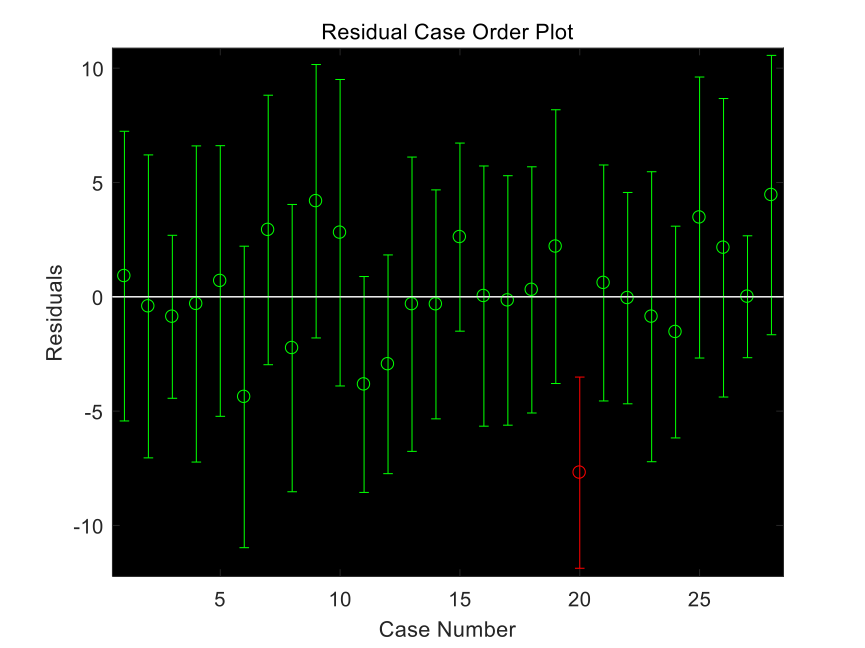
\includegraphics[width=\textwidth]{4-1.png}
\caption{白葡萄数据异常点}
\label{白葡萄数据异常点}
\end{figure}
\begin{figure}[htbp]
\centering
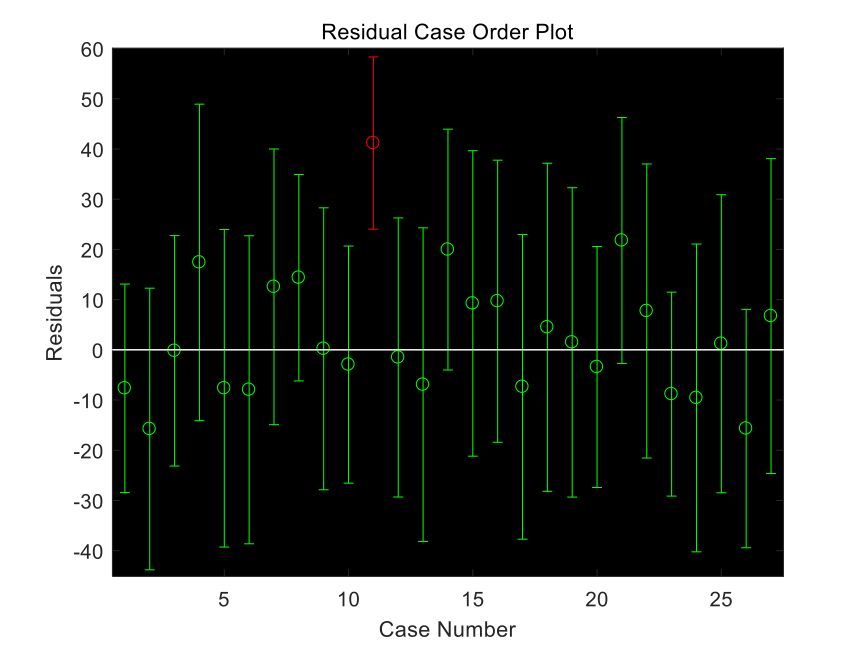
\includegraphics[width=\textwidth]{hongerr.png}
\caption{红葡萄数据异常点}
\label{红葡萄数据异常点}
\end{figure}

\subsubsection{排除异常值后再次进行回归,得到回归模型的系数}
\par 白葡萄:0.0340    0.1486   -0.3844    0.6852    0.3013    0.5350    0.5600    0.3459   -0.3300    1.4586    0.8932   -0.8804
\par 红葡萄:-0.0357   -0.5391    1.8852    0.0821    0.0003    1.1369   -0.1293   -3.4698    0.3069    0.5694

\subsubsection{对回归模型进行检验}
\par 首先进行残差的正态性检验:$A=jbtest(r)$,$B=ttest(r)$,若$A=0$,可认为以95\%的概率接受残差属于正态分布。反之,以95\%的概率拒绝原假设,认为残差不属于正态分布。若B=0,可认为以95\%的概率接受残差的均值为0。反之,以95\%的概率拒绝原假设,认为残差的均值不为0。因而这两个函数返回值都为0时,可认为回归较为合理。

\par 解得白葡萄:$A=0$,$B=0$;红葡萄:$A=0$,$B=0$。说明对于红葡萄和白葡萄而言,可认为回归所得残差均属于正态分布且均值为0。
\par 对线性模型和回归系数进行F检验:

\par 白葡萄:相关系数$r^2=0.6455$、$F=4.0252$、与$F$对应的概率$p=0.0071$,$\sigma^2=6.4161$,其中与F对应的概率$p=0.007<0.05$,回归模型成立。葡萄酒质量Y的结果如下公式(\ref{y1})所示。
\begin{equation}
\label{y1}
Y = 0.0340x_1 +  0.1486x_2 -0.3844x_3  +  0.6852x_4 +   0.3013x_5  +  0.5350x_6  +  \\
0.5600x_7 +   0.3459x_8   -0.3300x_9  +  1.4586x_{10} +  0.8932x_{11} -0.8804x_{12}
\end{equation}

\par 红葡萄:相关系数$r^2=-4.2395$、$F=2.0841$、与F对应的概率$p=0.0959$,$\sigma^2=107.7054$。

\par 其中与$F$对应的概率$p=0.09>0.05$,回归模型不好。考虑到第一个和第五个主成分的回归系数最小,分别只有$-0.03$和$0.0003$,筛去这两个主成分再次回归。

\par 新得到的相关系数$r^2=-4.2610$、$F=3.0627$、与$F$对应的概率$p=0.0262$,$\sigma^2=96.1310$,其中与$F$对应的概率$p=0.02<0.05$,回归模型成立。
\begin{equation}
	\label{y2}
Y=  -0.5259x_2 +   1.8335 x_3 +  0.1024x_4  +  1.0148x_6   -0.2798x_7   -3.5557x_8 +   0.2958x_9+    0.4338x_{10}
\end{equation}
\subsubsection{交叉验证结果}
\begin{table}[!htbp]
\centering
\caption{红葡萄交叉检验结果}
\label{红葡萄交叉检验结果}
\begin{tabular}{cccc}
\toprule
样品&评酒员评分值&交叉检验评分值&相对误差\\
\midrule
1&68.1&67.2694&0.012197\\
2&74&77.4371&0.046447\\
3&74.6&73.3657&0.016546\\
4&71.2&68.7095&0.034979\\
5&72.1&72.93622293&0.011598\\
6&66.3&70.4095683&0.061984\\
\bottomrule 
\end{tabular}
\end{table}

\begin{table}[!htbp]
\centering
\caption{白葡萄交叉检验结果}
\label{白葡萄交叉检验结果}
\begin{tabular}{cccc}
\toprule
样品&评酒员评分值&交叉检验评分值&相对误差\\
\midrule
1&77.9&75.7455&0.027657\\
2&75.8&77.44414366&0.021691\\
3&75.6&83.37830443&0.102888\\
4&76.9&78.03123828&0.014711\\
5&81.5&78.68851626&0.034497\\
6&75.5&78.57964869&0.04079\\
\bottomrule 
\end{tabular}
\end{table}

最终得到白葡萄交叉检验的平均相对误差为4.7\%。
综上我们可以得到可以通过酿酒葡萄的理化指标确定葡萄酒的质量。

\newpage
\section{模型优缺点}
\subsection{模型优点}
\begin{enumerate}
	\item 本文在对酿酒葡萄进行聚类时,采用K-means聚类的方法,从酿酒葡萄理化指标出发进行聚类,该聚类更加具有客观性
	\item 本文在对酿酒葡萄划分等级的时候,采用Fisher 函数的一般形式,确定葡萄酒质量划分为5个等级时为较优结果。
	\item 本文在酿酒葡萄的理化指标和葡萄酒理化指标关联的分析时,对酿酒葡萄的理化指标采取了主成分分析,即用较少的几个综合指标代替原有较多的变量的指标,而且使这些较少的综合指标既能尽量多的反应原来较多变量指标所反应的信息,简化了问题。
\end{enumerate}

\subsection{模型缺点}
\begin{enumerate}
	\item 由于本文在$K-means$聚类的过程中,直接利用统计软件$spss$进行计算,而没有考虑到变量的线性相关性。
	\item 本文对葡萄酒的质量只采取了葡萄酒的总评分的均值作为葡萄酒质量的衡量指标,并没有对葡萄酒的外观,香气,口感评分指标进行具体的分析。
\end{enumerate}



\section{模型改进方向}
\begin{enumerate}
	\item 在$K-means$聚类之前,我们应该对变量的线性相关性进行检验,将线性相关性高的变量进行合成或者剔除。
	\item 可以将葡萄酒的质量分成这三部分,用外观,香气,口感的评分均值分别衡量葡萄酒这三部分的质量,将葡萄酒质量细化。
\end{enumerate}


%参考文献
\begin{thebibliography}{9}%宽度9
 \bibitem{k-means} 袁方, 周志勇, 宋鑫. 初始聚类中心优化的k-means算法[J]. 计算机工程, 2007, 33(3):65-66.
 \bibitem{F检验} 陈希镇. F检验和信度系数α[J]. 数理统计与管理, 1993(1):37-41.
 \bibitem{Fisher} 曹苏群. 基于模糊Fisher准则的聚类与特征降维研究[D]. 江南大学, 2009.
 \bibitem{层次聚类} 尉景辉, 何丕廉, 孙越恒. 基于K-Means的文本层次聚类算法研究[J]. 计算机应用, 2005, 25(10):2323-2324. 
 \bibitem{主成分分析} 李艳双, 曾珍香, 张闽,等. 主成分分析法在多指标综合评价方法中的应用[J]. 河北工业大学学报, 1999, 28(1):94-97.
 \bibitem{baidu}url{https://baike.baidu.com/item/\%E8\%8A\%B1\%E8\%89\%B2\%E8\%8B\%B7/10868564?fr=aladdin}
\end{thebibliography}



\end{document} 